\chapter{Generative models}

\begin{description}
    \item[Generative model] \marginnote{Generative model}
        Model that tries to learn a probability distribution $p_\text{model}$ close to that of the data $p_\text{data}$.

        This can be done either by:
        \begin{itemize}
            \item Explicitly estimating the distribution.
            \item Building a generator to sample data from the distribution $p_\text{model}$ and possibly providing a likelihood.
        \end{itemize}

        \begin{remark}
            Generative models are suited for problems with multi-modal outputs (i.e. with no unique solution).
        \end{remark}

    \item[Latent variable model] \marginnote{Latent variable model}
        Given a vector of values $z$ with known prior distribution $P(z)$,
        a latent variable model expresses the probability of a data point $X$ (of the visible space) through marginalization over $z$:
        \[ P(X) = \int P(X|z) P(z) \,dz \approx \mathbb{E}_{z \sim P(z)} P(X|z) \]
        $z$ is considered the latent encoding of $X$ (usually it is some sort of noise).

        The network (generator) on input $z$ can either learn:
        \begin{itemize}
            \item The probability $P(X|z)$.
            \item To generate data points $\hat{X}$ (most likely) belonging to the distribution $P(X|z)$.
        \end{itemize} 

        \begin{figure}[H]
            \centering
            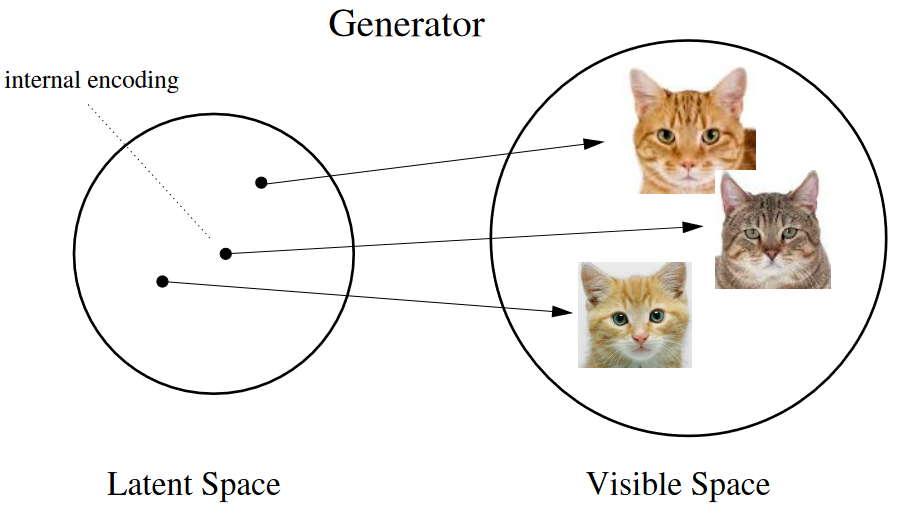
\includegraphics[width=0.45\linewidth]{./img/latent_space.png}
        \end{figure}
\end{description}

Generative models are categorized into two families:
\begin{descriptionlist}
    \item[Compressive models] \marginnote{Compressive models}
        Models where the latent space is smaller than the visible space.

    \item[Dimension-preserving models] \marginnote{Dimension-preserving models}
        Models where the latent space has the same dimension as the visible space.
\end{descriptionlist}

\begin{remark}
    Training latent variable models requires a way to encode the visible training data $X$ into their latent space $z$.
    Training relying only on the latent space does not make sense as, in this case, the output of the generator can be arbitrary.
\end{remark}



\section{Variational autoencoder (VAE)}

Model belonging to the family of compressive models.

\subsection{Training}

An autoencoder is modified in such a way that:
\begin{itemize}
    \item The encoder takes as input a visible data point $X$ and outputs its latent encoding $z$.
        The encoder is trained to force the marginal distribution of the latent space $Q(z) = \mathbb{E}_{X \sim P_\text{data} Q(z|X)}$ 
        into a known distribution (usually a standard Gaussian).

    \item The decoder (generator) takes as input the latent encoding $z$ of the encoder and outputs a reconstruction $\hat{X}$.
\end{itemize}

\begin{figure}[H]
    \centering
    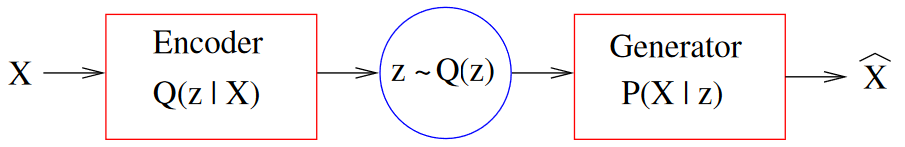
\includegraphics[width=0.5\linewidth]{./img/vae.png}
\end{figure}

It is assumed that for each different input $X$, $Q(z|X)$ has a different Gaussian distribution $G(\mu(X), \sigma(X))$
where both $\mu(X)$ and $\sigma(X)$ are computed by the encoder.

$z=\mu(X)$ can be seen as the latent encoding of $X$, 
while $\sigma(X)$ represents an area of the latent space around $z$ that encodes an information similar to $X$.

During training, the decoder receives in input a point sampled around $\mu(X)$ with variance $\sigma(X)$.

Two losses are used:
\begin{descriptionlist}
    \item[Reconstruction distance] 
        Aims to minimize the distance between the input $X$ and its reconstruction $\hat{X}$:
        \[ \Vert X - \hat{X} \Vert^2 \]

    \item[Kullback-Leibler divergence] 
        Aims to bring the marginal inference distribution $Q(z)$ close to a known distribution (e.g. a standard Gaussian):
        \[ \text{KL}[ Q(z | X) || P(z) ] = \text{KL}[ Q(z | X) || \mathcal{N}(0, 1) ] \]

        \begin{remark}
            The loss is applied to the single distributions $Q(z | X)$ but the effects are propagated to the marginal $Q(z)$.
        \end{remark}

        \begin{remark}
            An effect of this loss (with the standard Gaussian) is to:
            \begin{itemize}
                \item Push $\mu(X)$ towards 0 (i.e. occupying a small area of the latent space).
                \item Push $\sigma(X)$ towards 1 (i.e. making the latent variables have a larger coverage space to make it easier to generate new significant data).
            \end{itemize}
            \begin{figure}[H]
                \centering
                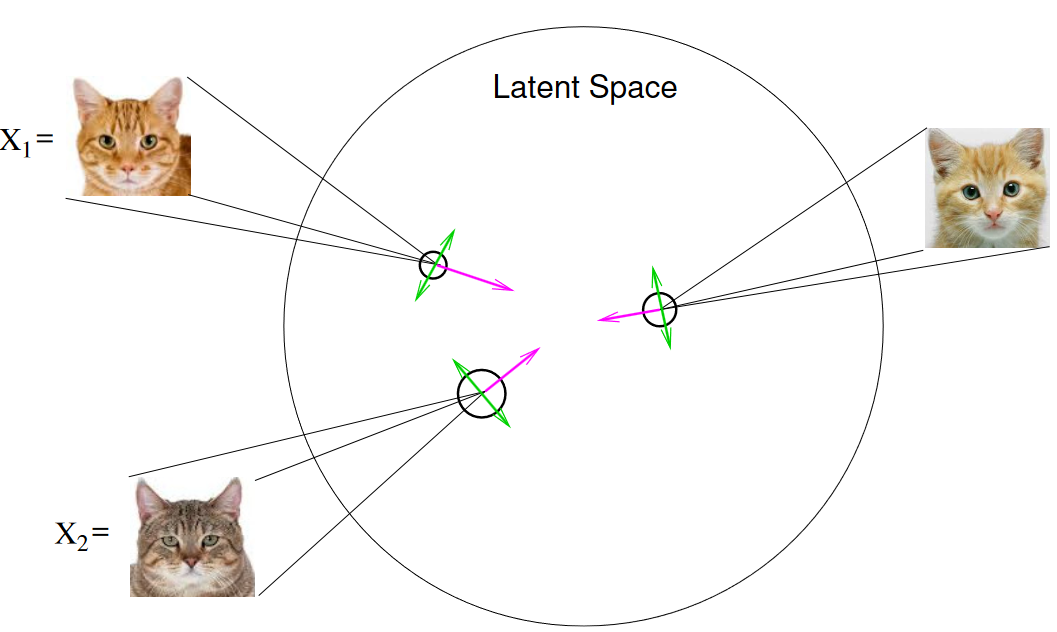
\includegraphics[width=0.4\linewidth]{./img/kl_vae.png}
                \caption{Effect of the KL-divergence on the latent space}
            \end{figure}
        \end{remark}
\end{descriptionlist}

\begin{figure}[H]
    \centering
    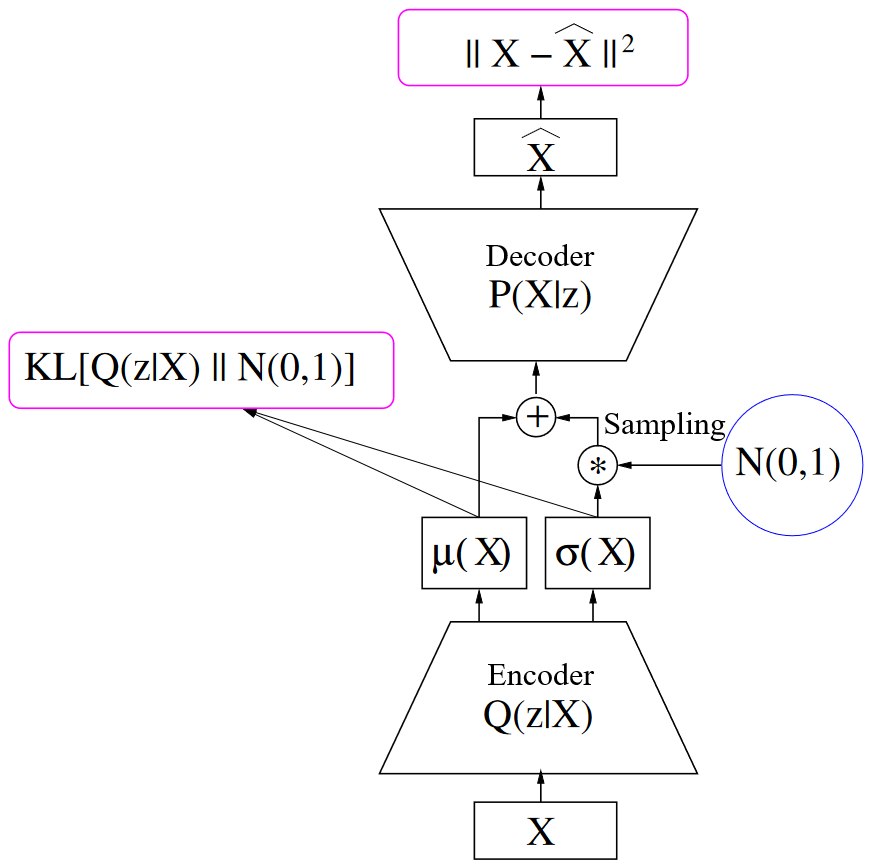
\includegraphics[width=0.4\linewidth]{./img/vae_training.png}
    \caption{Recap of the VAE training process}
\end{figure}



\subsection{Inference}

During inference, the encoder is not used as there are no visible input data $X$.
The decoder generates new data by simply taking as input a latent variable $z$ sampled from its prior distribution (e.g. a standard Gaussian).



\section{Generative adversarial network (GAN)}

Model belonging to the family of compressive models.

During training, the generator is paired with a discriminator that learns to distinguish between real data and generated data.

The loss function aims to:
\begin{itemize}
    \item Instruct the discriminator to spot the generator.
    \item Instruct the generator to fool the discriminator.
\end{itemize}

\begin{figure}[H]
    \centering
    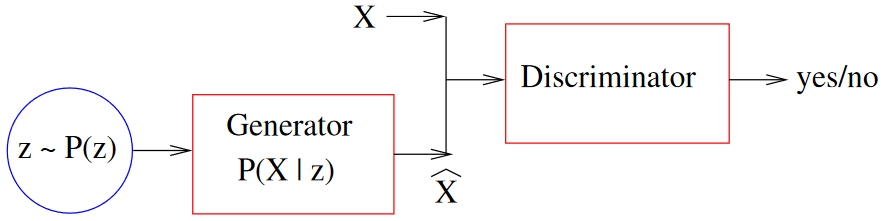
\includegraphics[width=0.5\linewidth]{./img/gan.png}
\end{figure}



\section{Normalizing flows}

Model belonging to the family of dimension-preserving models.

The generator is split into a chain of invertible transformations.
During training, the log-likelihood is maximized.

\begin{remark}
    Using only invertible transformations limits the expressiveness of the model.
\end{remark}

\begin{figure}[H]
    \centering
    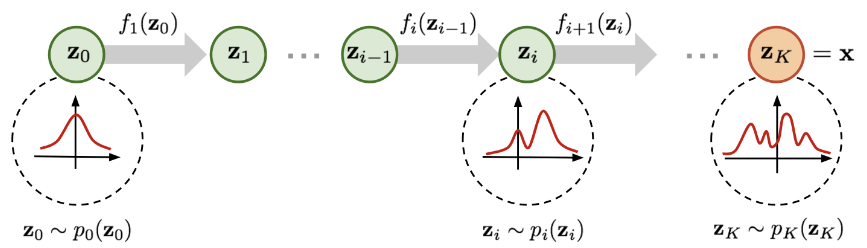
\includegraphics[width=0.65\linewidth]{./img/normalizing_flow.png}
\end{figure}



\section{Diffusion models}

Model belonging to the family of dimension-preserving models.

The generator is split into a chain of denoising steps that attempt to remove a Gaussian noise with varying $\sigma$.
It is assumed that the latent space is a noisy version of the image.

\begin{figure}[H]
    \centering
    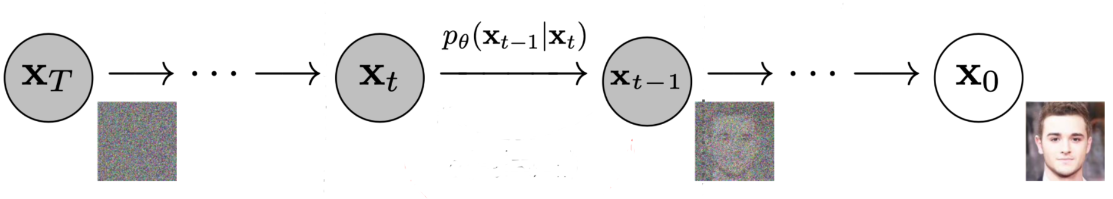
\includegraphics[width=0.65\linewidth]{./img/diffusion_model.png}
\end{figure}